% ****** Start of file apssamp.tex ******
%
%   This file is part of the APS files in the REVTeX 4.1 distribution.
%   Version 4.1r of REVTeX, August 2010
%
%   Copyright (c) 2009, 2010 The American Physical Society.
%
%   See the REVTeX 4 README file for restrictions and more information.
%
% TeX'ing this file requires that you have AMS-LaTeX 2.0 installed
% as well as the rest of the prerequisites for REVTeX 4.1
%
% See the REVTeX 4 README file
% It also requires running BibTeX. The commands are as follows:
%
%  1)  latex apssamp.tex
%  2)  bibtex apssamp
%  3)  latex apssamp.tex
%  4)  latex apssamp.tex
%
\documentclass[%
 reprint,
%superscriptaddress,
%groupedaddress,
%unsortedaddress,
%runinaddress,
%frontmatterverbose, 
%preprint,
%showpacs,preprintnumbers,
%nofootinbib,
%nobibnotes,
%bibnotes,
 amsmath,amssymb,
 aps,
%pra,
%prb,
%rmp,
%prstab,
%prstper,
%floatfix,
]{revtex4-1}

\usepackage{graphicx}% Include figure files
\usepackage{dcolumn}% Align table columns on decimal point
\usepackage[spanish]{babel}
\selectlanguage{spanish} 
\usepackage[utf8]{inputenc}
\usepackage{bm}% bold math
%\usepackage{hyperref}% add hypertext capabilities
%\usepackage[mathlines]{lineno}% Enable numbering of text and display math
%\linenumbers\relax % Commence numbering lines
\usepackage{float}
%\usepackage[showframe,%Uncomment any one of the following lines to test 
%%scale=0.7, marginratio={1:1, 2:3}, ignoreall,% default settings
%%text={7in,10in},centering,
%%margin=1.5in,
%%total={6.5in,8.75in}, top=1.2in, left=0.9in, includefoot,
%%height=10in,a5paper,hmargin={3cm,0.8in},
%]{geometry}
\usepackage[font=footnotesize,labelfont=bf]{caption}
\usepackage{hyperref}
\newcommand{\subtitle}[1]{%
\posttitle{%
    \par\end{center}
\begin{center}\large#1\end{center}
\vskip0.5em}%
}
\begin{document}

%\preprint{APS/123-QED}

\title{Bombeo óptico\\ \textit{Estudio del efecto Zeeman fuerte y débil sobre un núcleo de Rubidio } }% Force line breaks with \\

%\subtitle{Estudio de la dualidad de onda partícula}

\author{Jose Alejandro Montaña Cortés}
\email{ja.montana@uniandes.edu.co}
% \altaffiliation[Also at ]{Departamento de Física, Universidad de los Andes}
\author{Jesús David Rincón Puche}%
\email{jd.rincon883@uniandes.edu.co}
\affiliation{Departamento de Física, Universidad de los Andes}%

%\collaboration{}%\noaffiliation

\date{\today}% It is always \today, today,
             %  but any date may be explicitly specified

\begin{abstract}
En este laboratorio se hizo uso del método de ``bombeo óptico'' para estudiar el efecto Zeeman en el átomo de Rubidio (Rb), al estudiar la región de campos magnéticos débiles, se encontró una relación entre los factores de Landé del $^{87}Rb$ y el $^{85}Rb$ de  $1.59\pm  0.09$, lo cual concuerda con lo predicho por la teoría, pues al ser los factores de Landé $-1/2$ y $-1/3$ para el $^{85}Rb$ y el $^{87}Rb$ respectivamente, la razón entre estos valores. Adicional a esto se hizo un estudio de los periodos de oscilación de las oscilaciones de Rabi en función de la intensidad, con esto se comprobó que estos estados estudiados eran en efecto degenerados, otra vez al encontrar la relación de los factores de Landé, y el tiempo para entrar y salir de un estado excitado es muy corto, del orden de los milisegundos.


\end{abstract}
\maketitle
%\tableofcontents

%---------------------INTRODUCCIÓN------------------
\section{Introducción}
 El entendimiento de las propiedades cuánticas de los átomos, tales como los números cuánticos que caracterizan el momento angular de un núcleo atómico, resultan ser una parte fundamental de mecánica cuántica, pues estas propiedades determinan el comportamiento de los espectros y por ende proporcionan una forma de caracterizar los distintos elementos. El bombeo óptico, permite excitar electrones de los núcleos a distintos estados. En esta práctica se muestra como estados que aparentan ser degenerados, pueden ser separados gracias a la interacción del átomo con un campo magnético. Particularmente se toman núcleos de Rubidio (Rb) y se ponen a interactuar con un campo magnético. Debido a el efecto Zeeman, a medida que el campo magnético externo se incrementa, la separación entre los niveles se hace más notoria, lo cual permite su observación en un montaje experimental relativamente simple.
 Debido a las reglas de selección de la mecánica cuántica, existen un conjunto posibles de transiciones permitidas a las cuales electrones pueden acceder. Basado en esto y la intensidad de campo magnético aplicado, es posible determinar que tan grande será la separación entre los niveles que eran previamente degenerados.
 
 Adicionalmente, esto se puede realizar para varios átomos y así observar su efecto Zeeman y sus oscilaciones de Rabi. El primer fenómeno consiste en desdoblar los niveles atómicos de la energía, y por ello, de las líneas espectrales, cuando los átomos se colocan en un campo magnético~\cite{Zeeman}. El segundo, consiste en la dinámica de dos niveles con luz en presencia de un campo magnético constante. Esto posee lo denominado como "Frecuencia de Rabi" la cual es proporcional a la interacción de las partículas con el campo~\cite{teoria de rabi}. Para esta práctica se observan estos efectos en $^{87}Rb$ y el $^{85}Rb$.
 
 \section{Desarrollo Teórico}
 
 \subsection{Efecto Zeeman}
 
La energía del sistema cambia al introducir un campo magnético de la forma:

\begin{equation}
    \Delta E=-\Vec{\mu} \cdot \Vec{B}
\end{equation}

Dónde $\mu$ es el momento magnético del átomo y $B$, el campo magnético. En este caso, el momento angular total ($J$) está restringido a los valores del número cuántido $M$. De esta manera la energía se convierte en:

\begin{equation}
    \Delta E=g_f\mu_B B M,
    \label{energia}
\end{equation}

dónde $g_f$ es el factor de Landé y $\mu_B$ es el magnetón de Bohr. En este caso, los factores de Landé para los isotopos mencionados se calculan de la siguiente forma:

\begin{equation}
    g_f=g_j*[\frac{F(F+1)+J(J+1)-I(I+1)}{2F(F+1)}]
\end{equation}

\begin{equation*}
      g_j=1+\frac{J(J+1)+S(S+1)-L(L+1)}{2J(J+1)}.
\end{equation*}

Dónde $S$ es el momento angular de espín; $L$, el momento angular de órbita (por tanto, $J$ es $J=S+L$). Por otro lado, se deben incluir nuevos al hamiltoniano~\cite{cohen}, los cuales son el momento de espín nuclear, $I$ y el nuevo espín total $F$, el cual es definido como $F=I+J$.

Reemplazando los valores conocidos para el Rubidio, se obtiene que los factores de Landé son: $g_j=2$, para ambos isótopos y $g_f(^{87}Rb)=-1/2$ y el $g_f(^{85}Rb)=-1/3$.

Ya conocido estos, y un campo débil se puede aplicar la relación de Planck-Einstein ($E=hf$, dónde h es la constante de Planck y f,la frecuencia). para encontrar que las frecuencias para excitar el rubidio en sus orbitales son de 487 kHz y 700 kHz, para el $^{85}Rb$ y el $^{87}Rb$, respectivamente.

\subsection{Oscilaciones de Rabi}

Como se mencionó en la introducción, las oscilaciones de Rabi son la dinámica de dos niveles con luz en presencia de un campo magnético constante. La relación entre la frecuencia de Rabi, aplicacando la ecuación \eqref{energia} junto con la relación de Planck-Einstein, con un valor de $M$ igual a 1, se obtiene que la relación entre la frecuencia de Rabi y el campo magnético es:

\begin{equation}
    f_r=\frac{g_f\mu_B B}{h}
\end{equation}

Lo cual muestra que esta frecuencia está relacionada con la amplitud del campo magnético y no con la intensidad, porque $B$ no está al cuadrado.

% trim={<left> <lower> <right> <upper>}
%----MONTAJE EXPERIMENTAL--------
\section{Montaje experimental}
\subsection{Instrumento de medición.}
Para este experimento se hizo uso del aparato de ``optical pumping'' de la marca TechSpin. Este aparato cuanta con una lampara de descarga RF (Radio frequency), un filtro de interferencia, un polarizador lineal, un polarizador de cuarto de onda, una cámara con rubidio\footnote{El vapor cámara de absorción del rubidio está encerrada en un horno de plexiglass, el cual permitía controlar la temperatura y por ende la presión de vapor del rubidio.}, 2 lentes focalizadores y un detector óptico, tal configuración puede observarse en la figura \ref{montaje experimental}
\begin{figure}[h]
\center{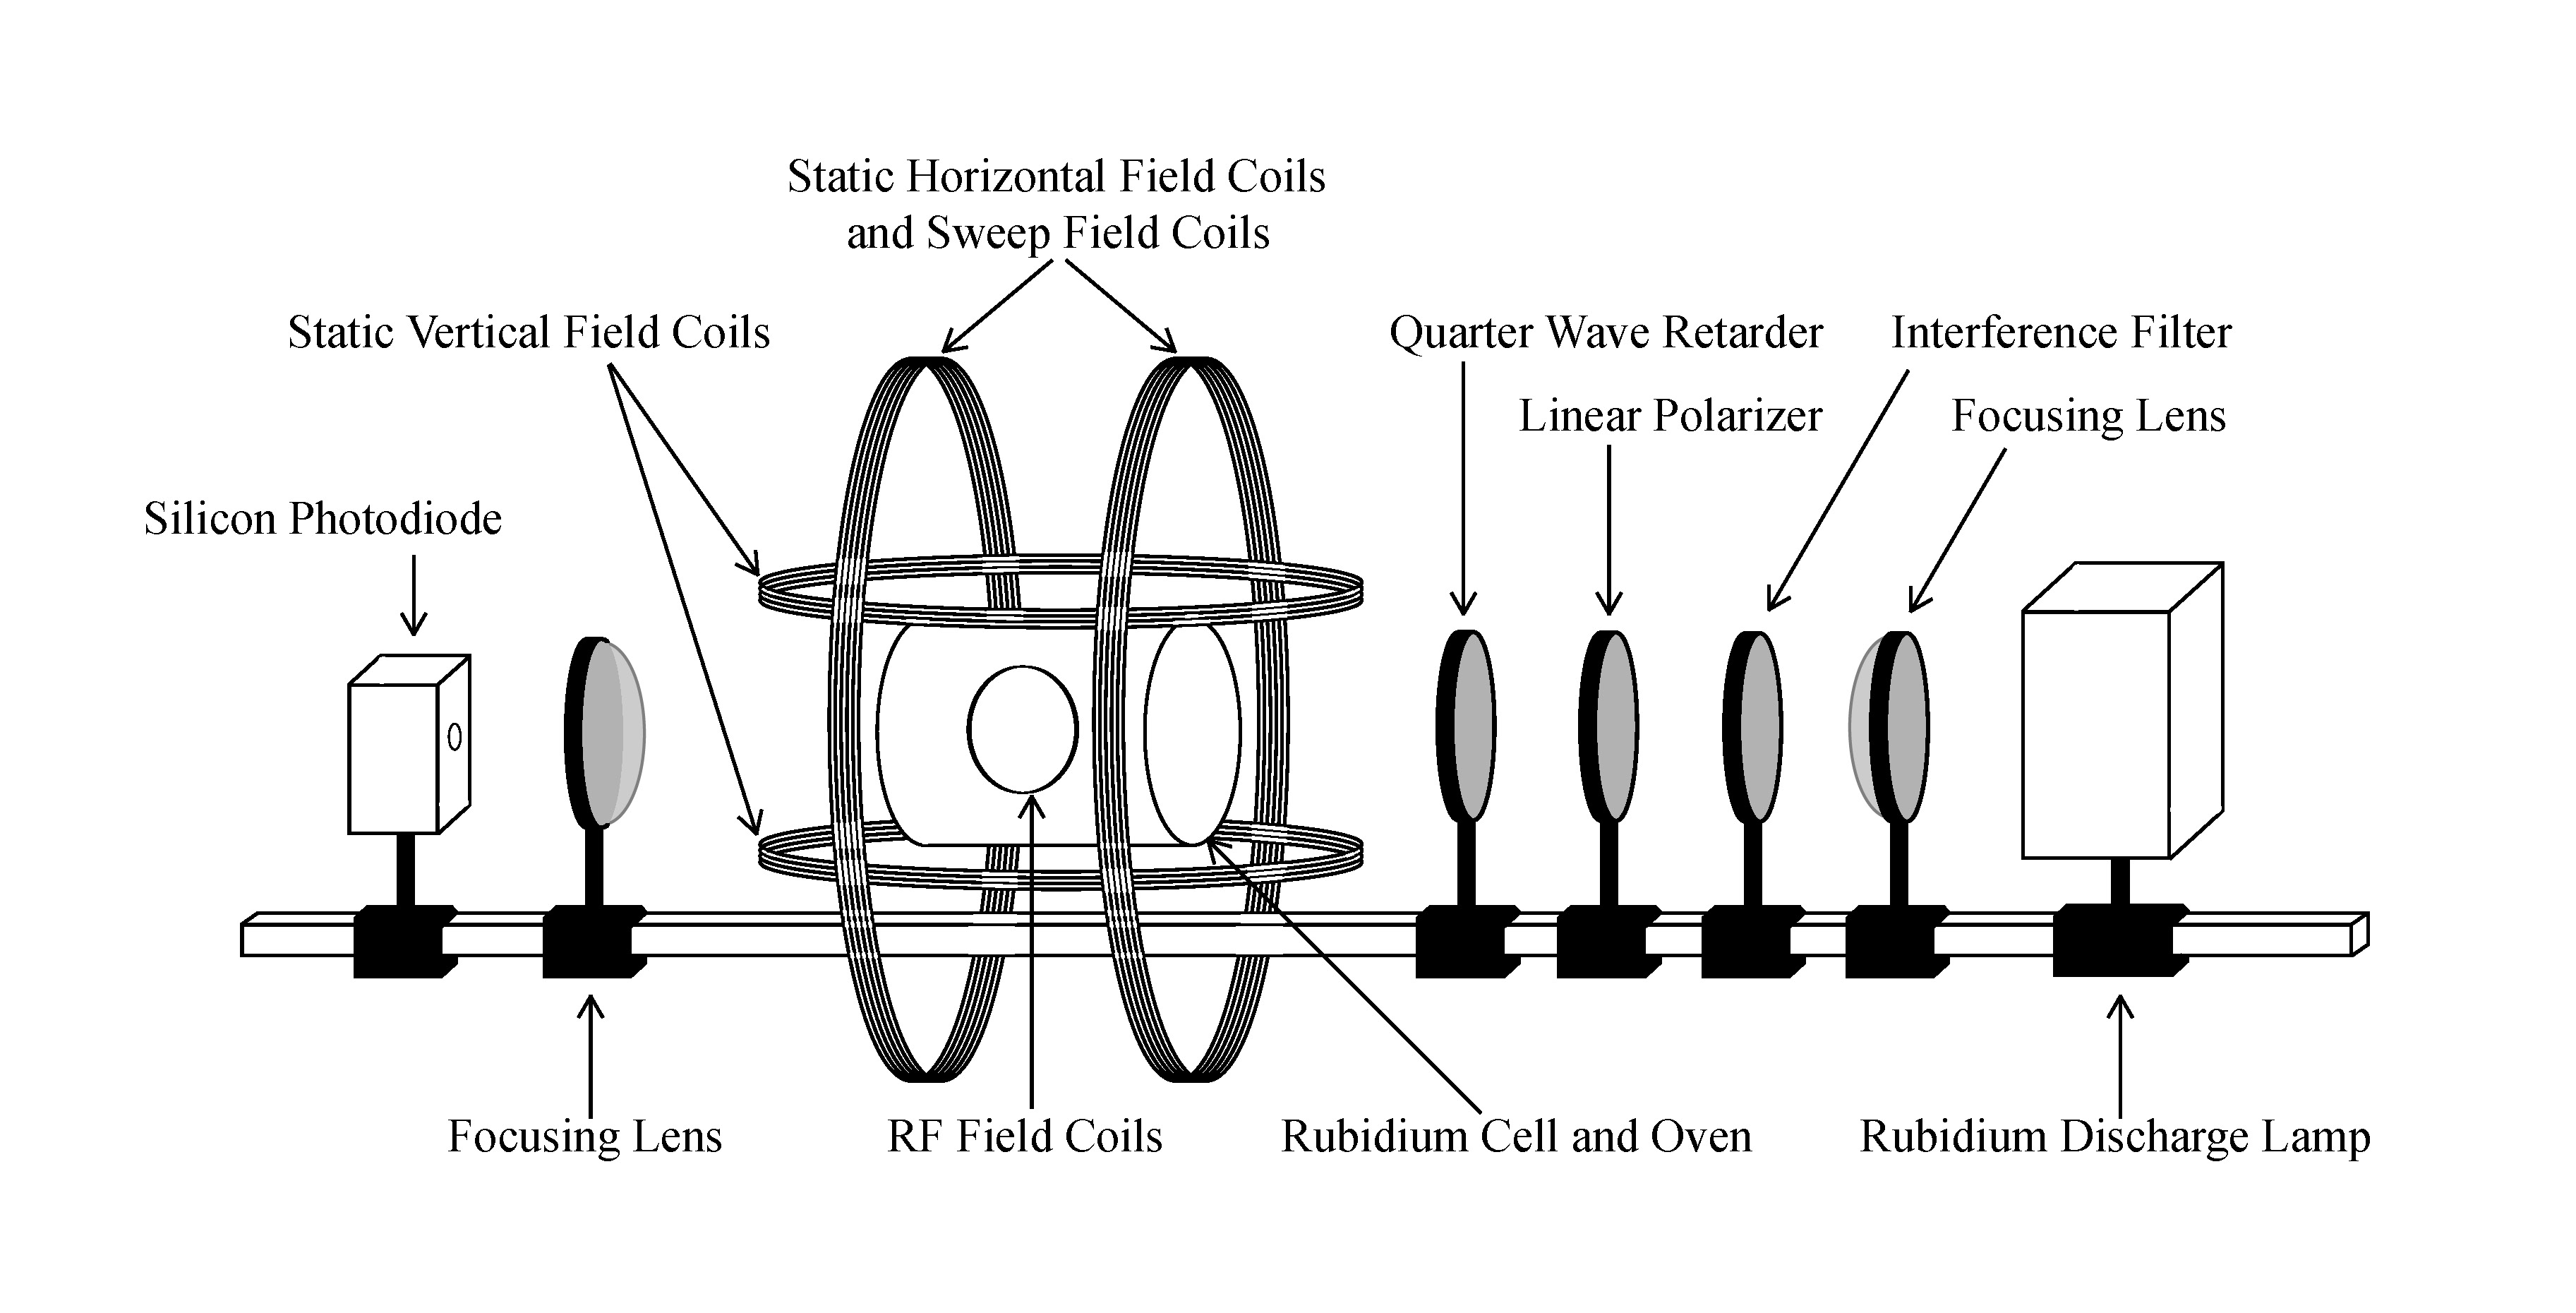
\includegraphics[width=0.4\textwidth]
{../Figuras/apparatus.jpg}}
\caption{\label{montaje experimental} Esquema del montaje experimental usado en este experimento.  (tomado de \cite{figura_aparato}).}
\end{figure}
La cámara en donde se encontraba el Rubidio estaba rodeada por 2 bobinas de Helmholtz para así producir los campos magnéticos. Uno de estos campos debe estar alineado con el campo magnético terrestre, configuración que se obtuvo haciendo uso de una brújula, esto con el fin de que el campo generado por las bobinas Helholtz contrarrestara el campo terrestre y así de esta forma calibrar nuestras mediciones. el otro conjunto de bobinas de Helmholtz es usado para crear un campo magnético de ``barrido'', el cual nos permite identificar la intensidad de los campos magnéticos en los cuales las transiciones ocurren.\\
El cable de RF es el encargado de revertir algunos de los efectos en el bombeo de los isótopos del Rb. Esto se logra al ajustar esta frecuencia en los estados que están siendo excitados.Para el caso del estado base, también se tiene que los fotones pueden ser absorbidos y por ende se observará una caída en la intensidad del detector.
\subsection{Configurando el aparato}
Con el fin de lograr visualizar los niveles de energía del rubidio se calibró inicialmente el montaje, tal que se asegurara una polarización circular de la luz, se puso el polarizador de media onda a un ángulo de 39 grados y con el fin de verificar que si se tenía polarización circular se dispuso un polarizador lineal al frente de la configuración (polarizador lineal y el de media onda), al ver que la intensidad en el detector no variaba al cambiar la disposición del último polarizador lineal, se concluyo que se estaba trabajando con polarización circular tal y como se requería. Seguido a esto se procedió a ajustar el campo magnético vertical en $0.1A$ y se fijó la ganancia en 200, luego se empezó a cambiar el valor del campo magnético de barrido para encontrar el valor de campo que producía el pico de transición que se buscaba. Una vez encontrada esta configuración se procedió a conectar el generador RF y se hizo un estudio del efecto de la radio frecuencia en función de la corriente a la cual se encontraban los picos. Por último se puso un generador de onda cuadrada y se ubicó uno de los picos anteriormente encontrados, la onda generada era de tipo cuadrada y y se dispuso un voltaje de $10V$ de pico a pico a una frecuencia de $5Hz$, esto con el fin de analizar los periodos generados en las oscilaciones de Rabi para cada uno de los picos, en esta parte se varió la intensidad de la radio frecuencia de entrada.\\
A continuación se muestran los resultados obtenidos.


%-----------------RESULTADOS----------------------
\section{Resultados y Análisis}
\subsection{Transición a campo cero}
En la primera parte se varió el campo de barrido dejando un campo magnético vertical a $0.1 A$, con lo cual se encontró que el pico en el cual se producía una transición se encontraba en $0.370A$, en la figura \ref{foto pico} se evidencia el comportamiento observado en el osciloscopio.

\begin{figure}[h]
\center{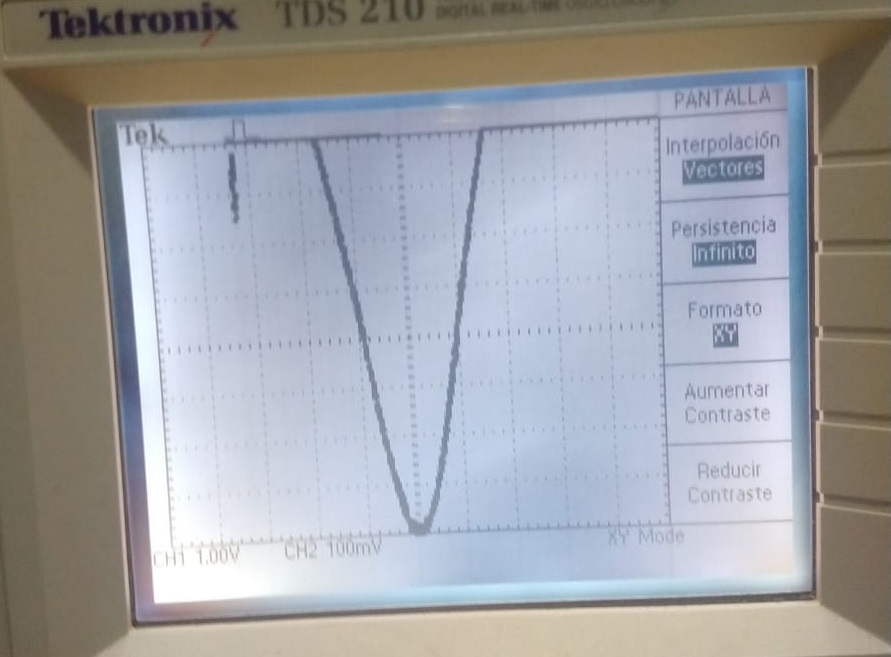
\includegraphics[width=0.4\textwidth,trim={0.3cm 0.5cm 0.3cm 0.5cm}]
{../Fotos/foto_pico.jpg}}
\caption{\label{foto pico} Imagen tomada en el momento del experimento, acá se muestra el pico que da razón de una transición entre 2 niveles de energía.}
\end{figure}
\begin{figure}[h]
\center{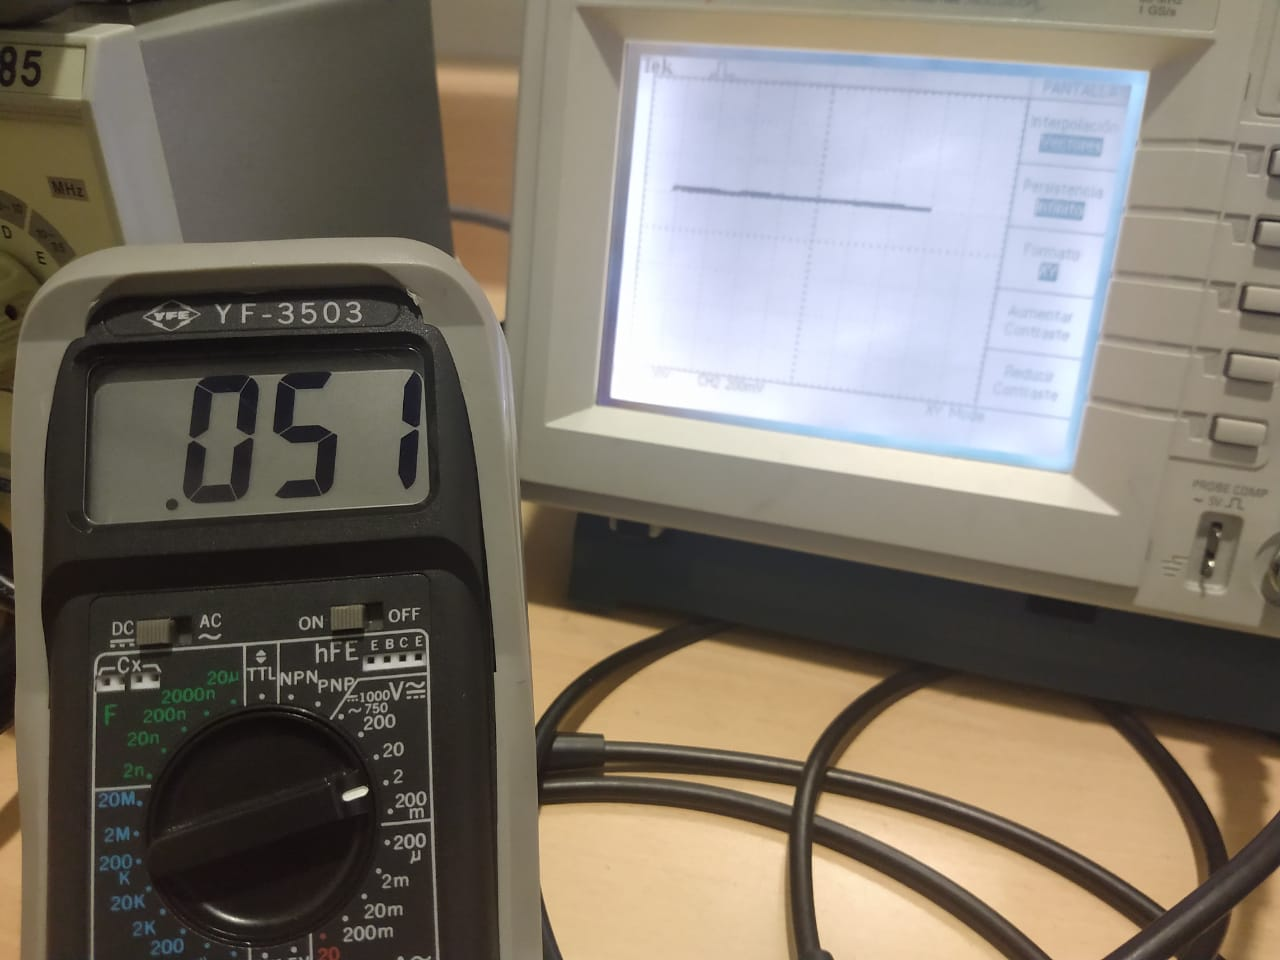
\includegraphics[width=0.4\textwidth,trim={0.3cm 0.5cm 0.3cm 0.5cm}]
{../Fotos/foto_muerto.jpeg}}
\caption{\label{foto muerto}  Imagen tomada en el momento del experimento, acá se aprecia la influencia de introducir un campo magnético horizontal externo.}
\end{figure}
De igual forma se varió el campo magnético horizontal para visualizar que influencia tenía este sobre el comportamiento en el pico, en la figura \ref{foto muerto} se observa que con tan sólo aumentar el campo magnético horizontal en $0.1 A$ el pico encontrado desaparece por completo. Esto se debe a que al poner una contribución externa de campo en otro dirección hace que los átomos no sean excitados de la misma forma y por ende esta transición desaparece.


\subsection{Efecto Zeeman para campo débil}

% trim={<left> <lower> <right> <upper>}
\begin{figure}[h]
\center{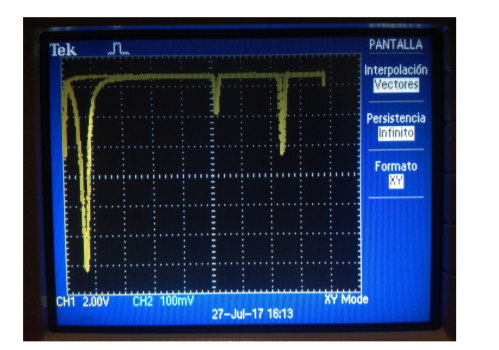
\includegraphics[width=0.4\textwidth,trim={0.1cm 0.3cm 0.1cm 0.3cm}]
{../Figuras/absorcionRb.PNG}}
\caption{Absorción de isótopos del Rubidio}
\label{absorcion}
\end{figure}

Como se observa en la figura \ref{absorcion}, la magnitud de los picos para cada isótopo es diferente. Esto significa que la intensidad de absorción de ellos pues la energía se puede relacionar con el potencial y al tener diferentes picos, es claro que no pueden ser iguales. Esto tiene sentido, dado que los isotopos tienen diferentes propiedades espín nuclear y niveles energéticos.
Una vez encontrado el valor de campo que produce el pico de transición, se procede a introducir una señal RF para así lograr identificar la separación de los niveles de energía de cada uno de los isótopos del Rubidio. Se varió la frecuencia y se observó como los picos variaban en función de esta frecuencia, en la figura \ref{feq_corr} se muestran los resultados obtenidos junto a los ajustes de cada conjunto de puntos.
% trim={<left> <lower> <right> <upper>}
\begin{figure}[h]
\center{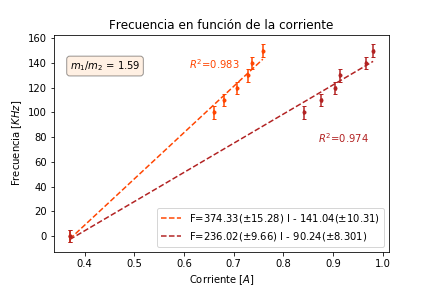
\includegraphics[width=0.4\textwidth,trim={0.1cm 0.3cm 0.1cm 0.3cm}]
{../Figuras/Freq_corr.png}}
\caption{\label{feq_corr} Ajuste al comportamiento entre la frecuencia aplicada y el valor del campo magnético en el cual se encontraba el pico. La linea anaranjada representa el primer isotopo del rubidio 87 mientras que la roja representa el Rubidio 85.}
\end{figure}
Como se observa en la figura \ref{feq_corr}, el comportamiento que se observa es de tipo lineal y además se tiene que la relación entre sus pendientes está muy cercano a lo esperado.
\begin{equation}
    \frac{m_{^{87}Rb}}{m_{^{85}Rb}}= 1.59\pm 0.09,
    \label{relacion_pendientes}
\end{equation}
así de esta forma se tiene entonces que la relación entre los factores de Landé ($g_F$) es cercana a la predicha por la teoría, con un 6\% de error comparado con el téorico, 1.5, el cual se obtiene de los factores de Landé reportados en la sección II.
\subsection{Oscilaciones de Rabi}

\begin{figure}[h]
\center{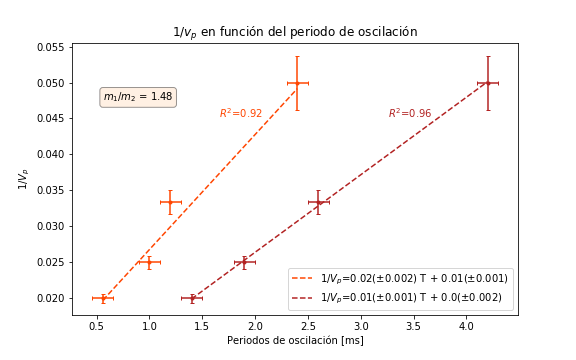
\includegraphics[width=0.4\textwidth,trim={0.1cm 0.3cm 0.1cm 0.3cm}]
{../Figuras/Voltaje_pp_periodo.png}}
\caption{\label{Volt_periodo} Ajuste lineal efectuado a los periodos de oscilación de Rabi en función del voltaje $V_{pp}$.}
\end{figure}
En la figura \ref{Volt_periodo} se muestra el ajuste efectuado entre el periodo encontrado en las oscilaciones de Rabi y el inverso del Voltaje, dado que la relación teórica entre el voltaje y la frecuencia es lineal\cite{teoria de rabi}, se esperaba que el ajuste entre el periodo y el inverso del voltaje fuera lineal.\\
Estas oscilaciones son debidas a la transición entre los niveles $M=2$ y $M=1$, aunque la práctica no nos permitió estudiar estos niveles de energía, puesto que no se efectuó la parte de efecto Zeeman cuadrático, el hecho de que se pueda visualizar estas oscilaciones nos da una idea de que el nivel de energía estudiado debe tener una degeneración, de forma que sea posible evidenciar este fenómeno. Esto último se observa al hacer las relaciones de las pendientes que dan 1.54, esta vez con un 2.7\% de error. 

Adicional a esto, se puede observar que el tiempo que le toma a un gas salir de un estado excitado a otro es muy corto, como se observa en~\ref{Volt_periodo}, y en el caso del $^{85}Rb$ es más grande esta excitación. Esto se puede deber a la absorción de este isótopo es más grande que la del otro.
%---------------CONCLUSIONES-------------------

\section{Conclusiones}
\begin{itemize}
    \item Se pudo lograr entender la idea del bombeo óptico. Esto se observa con la figura \ref{foto pico} porque muestra como a cierto valor de campo magnético débil, el rubidio es excitado. Se puede concluir que esto fue logrado por la luz que entraba en el horno del montaje así, alimentando a estos isótopos estudiados.
    \item Gracias a la imagen \ref{foto pico} se evidencian los fotones resonantes, porque ellos son los mediadores para el cambio de energía en la luz. Con respecto a los niveles de energía del espín núclear y el efecto Zeeman, estos se evidenciaron en las figuras \ref{absorcion} y \ref{feq_corr}. Ambas figuras nos confirmaron la teoría mencionada para los factores de Landé y el efecto Zeeman, porque al haber cumplido con la razón esperada, se puede afirmar un éxito en la observación de estos fenómenos, con un 6\% de error, lo que indica que los datos tomados son confiables. Para las oscilaciones de Rabi, sucede algo similar, pues en la figura \ref{Volt_periodo}, se obtiene también la relación esperada, con un 4\% de error.
\end{itemize}
%Se deben contestar las preguntas planteadas inicialmente o dar las razones por las cuales no es posible hacerlo. Las conclusiones deben ser necesariamente una consecuencia del experimento realizado, es decir que no se deben tocar aspectos que no se hayan expuesto en la sección de resultados y análisis. Si escribe algo que no se encuentra en la sección de resultados y análisis, esto quiere decir que hace falta incluir material en resultados y análisis. Concluir únicamente aspectos pertinentes a su trabajo en el laboratorio; evite generalizaciones que no hablan concretamente de lo que usted hizo o midió.

\begin{thebibliography}{9}
\bibitem{Zeeman}
Borda, N; Davidovich, I; Instituto Balseiro. Estudio del efecto Zeeman en Hg y determinación del magnetón de Bohr, 2009.
\bibitem{teoria de rabi}
\url{http://www.bgu.ac.il/atomchip/Theses/Amir_Waxman_MSc_2007.pdf}
\bibitem{cohen}
C. Cohen-Tannoudji, B. Diu, and F. Laloe. \textit{Quantum Mechanics}, 2 Volume Set. Wiley,1992.
\bibitem{figura_aparato}
\url{http://spa-mxpweb.spa.umn.edu/s11/Projects/S11_OpticalPumping/apparatus.htm}
\bibitem{guia optical pumping}
Mejía, J; Universidad de los Andes. \textit{Bombeo óptico}, 2017.

\end{thebibliography}

\end{document}
%
% ****** End of file apssamp.tex ******

